\begin{tabular}{c | c | c | c}
	Art & Literatur & Berechnet & Abweichung \\
	\hline
	Rund & \SI{10e+10}{\newton\per\metre\squared} & \SI{5.29(4)e+10}{\newton\per\metre\squared} & -52.9\% \\
	Eckig & \SI{7e+10}{\newton\per\metre\squared} &\SI{7.37(5)e+10}{\newton\per\metre\squared} & +5.3\%\\
	Beidseitig links & \SI{7e+10}{\newton\per\metre\squared} & \SI{18.0(6)e+10}{\newton\per\metre\squared} & +157.1\% \\
	Beidseitig rechts & \SI{7e+10}{\newton\per\metre\squared} & \SI{13.8(6)e+10}{\newton\per\metre\squared} & +97.1\% \\
\end{tabular} \\
Für Messing stand auf Wikipedia $(78-123)\cdot\SI{e+9}{\newton\per\metre\squared}$. \\
Für Aluminium $\SI{70e+9}{\newton\per\metre\squared}$.

\ \\
\ \\

\begin{tabular}{c | c | c | c | c}
	Abstand von der Mitte & links mit & rechts mit & links ohne & rechts ohne \\
	in cm & in mm & in mm & in mm & in mm \\
	\hline
	3.75 & 6.320 & 7.125 & 7.620 & 8.320 \\
	4.25 & 6.325 & 7.160 & 7.625 & 8.310 \\
	4.75 & 6.320 & 7.200 & 7.635 & 8.310 \\
	5.25 & 6.325 & 7.230 & 7.610 & 8.300 \\
	5.75 & 6.330 & 7.250 & 7.600 & 8.320 \\
	6.25 & 6.330 & 7.295 & 7.595 & 8.340 \\
	6.75 & 6.340 & 7.345 & 7.600 & 8.365 \\
	7.25 & 6.340 & 7.395 & 7.610 & 8.380 \\
	7.75 & 6.360 & 7.420 & 7.585 & 8.390 \\
	8.25 & 6.350 & 7.450 & 7.580 & 8.450 \\
	9.25 & 6.400 & 7.510 & 7.570 & 8.395 \\
	10.25 & 6.420 & 7.610 & 7.560 & 8.430 \\
	11.25 & 6.455 & 7.700 & 7.560 & 8.465 \\
	12.25 & 6.480 & 7.760 & 7.560 & 8.460 \\
	13.25 & 6.570 & 7.830 & 7.600 & 8.470 \\
	15.25 & 6.750 & 7.950 & 7.650 & 8.450 \\
	17.25 & 6.920 & 8.060 & 7.700 & 8.450 \\
	19.25 & 7.135 & 8.155 & 7.790 & 8.405 \\
	21.25 & 7.370 & 8.250 & 7.880 & 8.430 \\
	23.25 & 7.595 & 8.285 & 7.960 & 8.360 \\
	25.25 & 8.010 & 8.230 & 8.150 & 8.280 \\
\end{tabular}
\ \\
\ \\
Die mittlere Biegung des Stabes ohne Gewicht
\begin{align*}
	D_\text{links} &= \SI{7.669(33)e-3}{\metre} \\
	D_\text{rechts} &= \SI{8.385(13)e-3}{\metre}
\end{align*}

\begin{figure}[h!]
	\centering
	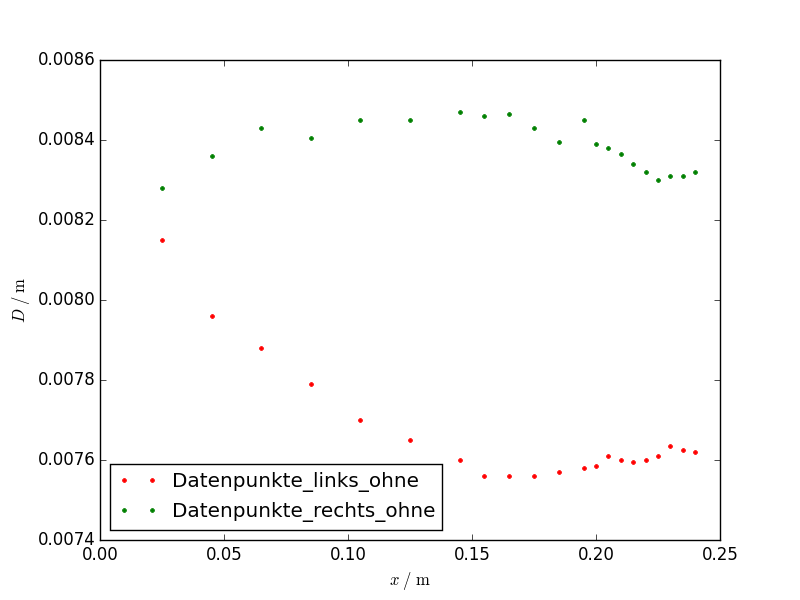
\includegraphics[width=\textwidth]{Werte_ohne.png}
	\caption{Messwerte für D und x ohne Gewicht}
\end{figure}
\begin{figure}[h!]
	\centering
	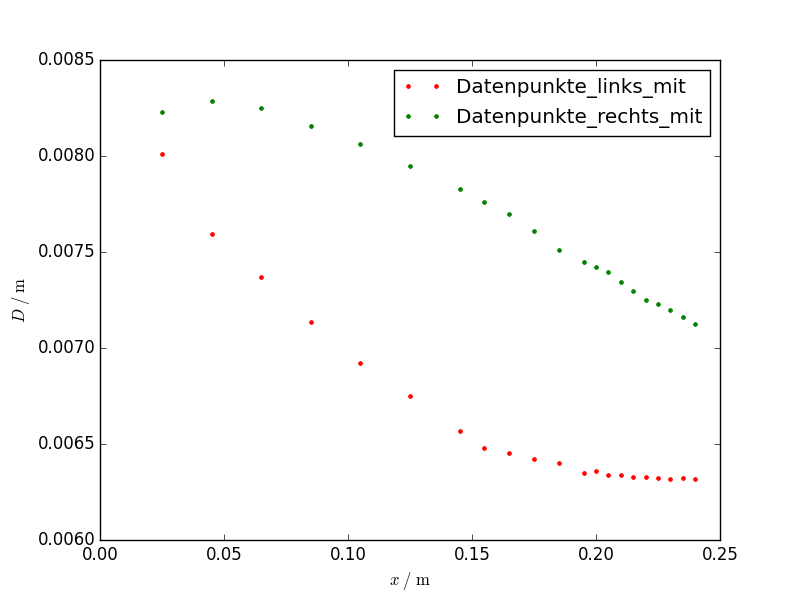
\includegraphics[width=\textwidth]{Werte_mit.png}
	\caption{Messwerte für D und x mit Gewicht}
\end{figure}
\begin{figure}[h!]
	\centering
	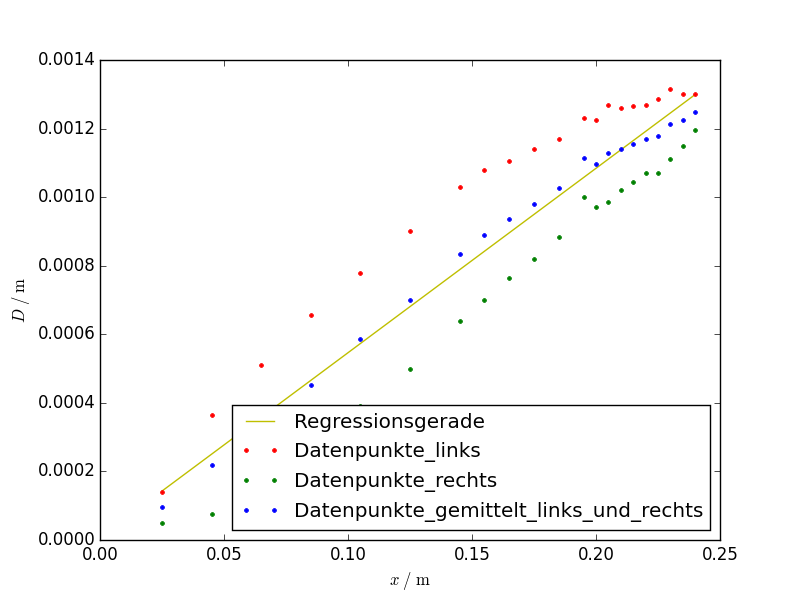
\includegraphics[width=\textwidth]{Wertedifferenz.png}
	\caption{Wirkliches D und x}
\end{figure}
